%%%%%%%%%%%%%%%%%%%%%%%%%%%%%%%%%%%%%%%%%%%
%
% From a template maintained at https://github.com/jamesrobertlloyd/cbl-tikz-poster
%
% Code near the top should be fairly standard and not need to be changed
%  - except for the document class
% Code lower down is more likely to be customised
%
%%%%%%%%%%%%%%%%%%%%%%%%%%%%%%%%%%%%%%%%%%%

%%%%%%%%%%%%%%%%%%%%%%%%%%%%%%%%%%%%%%%%%%%
%
% Document class
%
% Change this if you want a different size / orientation poster etc
%
%%%%%%%%%%%%%%%%%%%%%%%%%%%%%%%%%%%%%%%%%%%

\documentclass[landscape,a0b,final,a4resizeable]{a0poster}
%\documentclass[portrait,a0b,final,a4resizeable]{a0poster}

%%%%%%%%%%%%%%%%%%%%%%%%%%%%%%%%%%%%%%%%%%%
%
% 'Basic' packages
%
% TODO - Almost certainly some are unnecessary - feel free to remove nonstandard
% packages if you think it is a good idea not to always have them
%
%%%%%%%%%%%%%%%%%%%%%%%%%%%%%%%%%%%%%%%%%%%

\usepackage{multicol}
\usepackage{color}
\usepackage{shadow}
\usepackage{morefloats}
\usepackage{cite}
\usepackage[pdftex]{graphicx}
\usepackage{rotating}
\usepackage{amsmath, amsthm, amssymb, bm}
\usepackage{array}
\usepackage{nth}
\usepackage[square,numbers]{natbib}
\usepackage{booktabs}

%%%%%%%%%%%%%%%%%%%%%%%%%%%%%%%%%%%%%%%%%%%
%
% TIKZ packages and common definitions
%
% Add extra things as per your tikz needs
%
%%%%%%%%%%%%%%%%%%%%%%%%%%%%%%%%%%%%%%%%%%%

\usepackage{../common/picins}
\usepackage{tikz}
\usetikzlibrary{shapes.geometric,arrows,chains,matrix,positioning,scopes,calc}
\tikzstyle{mybox} = [draw=white, rectangle]

%%%%%%%%%%%%%%%%%%%%%%%%%%%%%%%%%%%%%%%%%%%
%
% myfig
%
% \myfig - replacement for \figure
% necessary, since in multicol-environment 
% \figure won't work        
%                 
%%%%%%%%%%%%%%%%%%%%%%%%%%%%%%%%%%%%%%%%%%%

\newcommand{\myfig}[3][0]{
\begin{center}
  \vspace{1.5cm}
  \includegraphics[width=#3\hsize,angle=#1]{#2}
  \nobreak\medskip
\end{center}}

%%%%%%%%%%%%%%%%%%%%%%%%%%%%%%%%%%%%%%%%%%%
%
% mycaption                
%
% \mycaption - replacement for \caption
% necessary, since in multicol-environment \figure and
% therefore \caption won't work
%
%%%%%%%%%%%%%%%%%%%%%%%%%%%%%%%%%%%%%%%%%%%

%\newcounter{figure}
\setcounter{figure}{1}
\newcommand{\mycaption}[1]{
  \vspace{0.5cm}
  \begin{quote}
    {{\sc Figure} \arabic{figure}: #1}
  \end{quote}
  \vspace{1cm}
  \stepcounter{figure}
}

%%%%%%%%%%%%%%%%%%%%%%%%%%%%%%%%%%%%%%%%%%%
%
% Some standard colours
%
%%%%%%%%%%%%%%%%%%%%%%%%%%%%%%%%%%%%%%%%%%%

\definecolor{camlightblue}{rgb}{0.601 , 0.8, 1}
\definecolor{camdarkblue}{rgb}{0, 0.203, 0.402}
\definecolor{camred}{rgb}{1, 0.203, 0}
\definecolor{camyellow}{rgb}{1, 0.8, 0}
\definecolor{lightblue}{rgb}{0, 0, 0.80}
\definecolor{white}{rgb}{1, 1, 1}
\definecolor{whiteblue}{rgb}{0.80, 0.80, 1}

%%%%%%%%%%%%%%%%%%%%%%%%%%%%%%%%%%%%%%%%%%%
%
% Some look and feel definitions
%
%%%%%%%%%%%%%%%%%%%%%%%%%%%%%%%%%%%%%%%%%%%

\setlength{\columnsep}{0.03\textwidth}
\setlength{\columnseprule}{0.0018\textwidth}
\setlength{\parindent}{0.0cm}

%%%%%%%%%%%%%%%%%%%%%%%%%%%%%%%%%%%%%%%%%%%
%
% \mysection - replacement for \section*
% 
% Puts a pretty box around some text
% TODO - any other thoughts for what this box should look like
%
%%%%%%%%%%%%%%%%%%%%%%%%%%%%%%%%%%%%%%%%%%%

\tikzstyle{mysection} = [rectangle, 
									draw=none, 
									shade, 
									outer color=camlightblue!30,
									inner color=camlightblue!30,
									text width=0.965\columnwidth,
									text centered,
									rounded corners=20pt,
									minimum height=0.11\columnwidth]

\newcommand{\mysection}[1]
{
\begin{center}
  \begin{tikzpicture}
    \node[mysection] {\sffamily\bfseries\LARGE#1};
  \end{tikzpicture}
\end{center}
}

%%%%%%%%%%%%%%%%%%%%%%%%%%%%%%%%%%%%%%%%%%%
%
% Set the font
%
% TODO - Not sure what a canonical choice is - feel free to modify
%
%%%%%%%%%%%%%%%%%%%%%%%%%%%%%%%%%%%%%%%%%%%

\renewcommand{\familydefault}{cmss}
\sffamily

%%%%%%%%%%%%%%%%%%%%%%%%%%%%%%%%%%%%%%%%%%%
%
% Poster environment
%
% Centres everything and can be used to define the width of the content
%
%%%%%%%%%%%%%%%%%%%%%%%%%%%%%%%%%%%%%%%%%%%

\newenvironment{poster}{
  \begin{center}
  \begin{minipage}[c]{0.96\textwidth}
}{
  \end{minipage} 
  \end{center}
}

%%%%%%%%%%%%%%%%%%%%%%%%%%%%%%%%%%%%%%%%%%%
%
% This is probably a good place to put content specific packages and definitions
%
%%%%%%%%%%%%%%%%%%%%%%%%%%%%%%%%%%%%%%%%%%%

\newtheorem{thm}{Theorem}%[section]
\newtheorem{lem}[thm]{Lemma}
\newtheorem{prop}[thm]{Proposition}
\newtheorem{cor}[thm]{Corollary}

\newtheorem*{theorem*}{Theorem}

\theoremstyle{definition}
\newtheorem*{definition*}{Definition}
\newtheorem{definition}[thm]{Definition}%[section]
\newtheorem{conj}{Conjecture}[section]
\newtheorem{exmp}{Example}[section]
\newtheorem{rem}[thm]{Remark}

\theoremstyle{remark}
%\newtheorem{rem}{Remark}
\newtheorem{note}{Note}
\newtheorem{case}{Case}

\newcommand{\eqd}{\overset{\,_{\!d}}{=}}
\newcommand{\defn}[1]{\emph{#1}}

\newcommand{\Law}{\mathcal{L}}

\def\given{\,|\,}

\def\SGinf{\mathbb{S}_{\infty}}

\newcommand{\NonNegInts}{\mathbb{Z}_+}
\newcommand{\Nats}{\mathbb{N}}
\newcommand{\Rationals}{\mathbb{Q}}
\newcommand{\Reals}{\mathbb{R}}

\newcommand{\as}{\textrm{a.s.}}

\def\[#1\]{\begin{align}#1\end{align}}
\newcommand{\defas}{:=}

\newcommand{\Normal}{\mathcal{N}}
\newcommand{\dist}{\ \sim\ }

\newcommand{\kernel}{\kappa}
\newcommand{\kernelmatrix}{K}
\newcommand{\scalefactor}{s}
\newcommand{\lengthscale}{\ell}
\newcommand{\targets}{T}
\newcommand{\noise}{\sigma_\targets}
\newcommand{\pseudopoints}{\eta}
\newcommand{\inputpoints}{\xi}
\newcommand{\covhyppar}{\psi}
\newcommand{\logistic}{\phi}

\newcommand{\CompOrder}{\mathcal{O}}
\def\graphspace{\mathbf{G}}
\def\Uniform{\mbox{\rm Uniform}}
\def\Bernoulli{\mbox{\rm Bernoulli}}
\def\ie{i.e.,\ }
\def\eg{e.g.,\ }
\def\iid{i.i.d.\ }
\def\simiid{\sim_{\mbox{\tiny iid}}}
\def\simind{\sim_{\mbox{\tiny ind}}}
\def\eqdist{\stackrel{\mbox{\tiny d}}{=}}
\def\ahfunction{\theta}       
\def\AHfunction{\Theta}           % A-H random function
\def\AHvar{U}                     % A-H uniform variables
\def\AHvaralt{V}                  % A-H uniform variables - for bipartite data
\def\larray{W}                    % latent array sampled with A-H
%\def\latentspace{\mathbf{W}}      % range of entries
\def\latentspace{\mathcal{W}}      % range of entries
\def\darray{X}                    % data array
%\def\dataspace{\mathbf{X}}        % sample space
\def\dataspace{\mathcal{X}}        % sample space
\def\cfspace{\mathbf{C}}          % space of continuous functions
%\def\GP{\mbox{\mathcal{GP}}}
\def\GP{\mathcal{GP}}
\def\likelihood{P}
\def\CovData{C}
\def\CovDataAlt{D}

\def\newarrow{\mbox{\begin{tikzpicture}
             \useasboundingbox{(-3pt,-4.5pt) rectangle (19pt,1pt)};
             \draw[->] (0,-0.07)--(17pt,-0.07);\end{tikzpicture}}}

%%%%%%%%%%%%%%%%%%%%%%%%%%%%%%%%%%%%%%%%%%%
%
% The document environment starts here
%
%%%%%%%%%%%%%%%%%%%%%%%%%%%%%%%%%%%%%%%%%%%

\begin{document}

%%%%%%%%%%%%%%%%%%%%%%%%%%%%%%%%%%%%%%%%%%%
%
% Begin the poster environment - centres things and potentially changes the width
%
%%%%%%%%%%%%%%%%%%%%%%%%%%%%%%%%%%%%%%%%%%%

\begin{poster}

%%%%%%%%%%%%%%%%%%%%%%%%%%%%%%%%%%%%%%%%%%%
%
% Potentially add some space at the top of the poster
%
%%%%%%%%%%%%%%%%%%%%%%%%%%%%%%%%%%%%%%%%%%%

\vspace{0\baselineskip}

%%%%%%%%%%%%%%%%%%%%%%%%%%%%%%%%%%%%%%%%%%%
%
% Draw the header as a TIKZ picture
%
% Using TIKZ to allow for easy alignment
%
%%%%%%%%%%%%%%%%%%%%%%%%%%%%%%%%%%%%%%%%%%%

\begin{center}
\begin{tikzpicture}[x=0.5\textwidth]
    % Dummy nodes at edges for spacing
    % TODO - a better way?
    \node at (+1, 0) {};    
    \node at (-1, 0) {};
    % Set the size of the badges
    \def \badgeheight {0.08\textwidth}
    % Title text
    \node[inner sep=0,text width=0.5\textwidth,text centered,font=\Huge] (Title) at (0,0) 
    {
      {\sffamily \Huge \textbf{A Bandit Framework for Optimal Selection of Reinforcement Learning Agents}}\\
      {\huge\sffamily Andreas Merentitis\textsuperscript{1}, Kashif Rasul\textsuperscript{2}, Roland Vollgraf\textsuperscript{2}, Abdul-Saboor Sheikh\textsuperscript{2}, Urs Bergmann\textsuperscript{2}}\\
      \vspace{-0.3\baselineskip}
      {\large\sffamily 1: OLX Berlin Hub, Germany, 2: Zalando Reasearch, Berlin, Germany}
    };
    % Cambridge badge
    \node [mybox] (NIPS Badge) at (-0.9, 0) {
        \includegraphics[\badgeheight]{../badges/ZalandoR.png}
    };
    % CBL badge
    \node [mybox] (CBL Badge) at (-0.6, 0) {
        \includegraphics[width=0.1\textwidth]{../badges/OLX_LogoHR_black.png}
    };
    % Columbia logo
    \node [mybox] (box) at (0.85, 0) {
        
\includegraphics[width=0.1\textwidth]{../badges/nips_small.png}
    };
\end{tikzpicture}
\end{center}

%%%%%%%%%%%%%%%%%%%%%%%%%%%%%%%%%%%%%%%%%%%
%
% Spacing between title and main body
%
%%%%%%%%%%%%%%%%%%%%%%%%%%%%%%%%%%%%%%%%%%%

\vspace{1\baselineskip}

%%%%%%%%%%%%%%%%%%%%%%%%%%%%%%%%%%%%%%%%%%%
%
% Columns environment
%
%%%%%%%%%%%%%%%%%%%%%%%%%%%%%%%%%%%%%%%%%%%

\begin{multicols}{3}

%%%%%%%%%%%%%%%%%%%%%%%%%%%%%%%%%%%%%%%%%%%
%
% Start of content
%
%%%%%%%%%%%%%%%%%%%%%%%%%%%%%%%%%%%%%%%%%%%

\large

\mysection{Motivation}

\vspace{0\baselineskip}

{\Large

\begin{itemize}
\item The optimal inductive bias (architecture, hyperparameters, etc.) of a RL agent depends on the application. 
\item We propose a multi-arm bandit with the double objective of maximizing the reward while the agents are learning and selecting the best agent after a small number of learning steps. 
\end{itemize}

}

\mysection{Multi-arm bandit framework}

Different types of bandit strategies are possible, from simple $\epsilon$-greedy, to techniques like SoftMax (probability matching bandit), UCB1 (based on the optimism in the face of uncertainty principle) and EXP3 (adversarial bandit). 

\begin{itemize}
\item It has been shown in [Yi-Sun-2011] that it is 
beneficial for agents to take actions that maximize the reduction in uncertainty about the environment dynamics
\item This can be formalized as taking a sequence of actions $a_t$ that maximize the sum of reductions in entropy.
\end{itemize}

With the history of the agents up until time step $t$ as $\xi_{t} = \{s_1 , a_1 , \dots , s_t \}$, we can write the sum of entropy reductions as:

\begin{equation}
        \sum_{t} \left( H\left(\bold\mathbf{\Theta}| \xi_{t}, a_t \right) - H \left(\bold\mathbf{\Theta} | S_{t+1}, \xi_{t}, a_t \right) \right). \label{eq:1}
\end{equation}

As indicated in [Houthooft-2018], according to information theory, the individual terms express the mutual information between the next state distribution $S_{t+1}$ 
and the model parameter distribution $\bold\mathbf{\Theta}$, namely $I(S_{t+1}; \bold\mathbf{\Theta}|\xi_{t},a_{t})$. This mutual information can be written as:

\begin{equation}
       I \left (S_{t+1};\bold\mathbf{\Theta}|\xi_{t},a_{t} \right) = \mathbb{E}_{s_{t+1} \sim P \left(\cdot|\xi_{t},a_{t} \right)} [D_{KL}[p \left(\theta|\xi_{t},a_t,s_{t+1}\right) || p \left(\theta|\xi_{t} \right)]], \label{eq:2}
\end{equation}

\begin{itemize}
\item the KL divergence term is expressing the difference between the new and the old beliefs of the agent regarding the environment dynamics, and the expectation is with respect
\item Under these assumptions the above formulation can also be interpreted as information gain [Houthooft-2018]
\end{itemize}

\mysection{Calculating the information gain}

Formally, since calculating the posterior $p(\theta|D)$ for a dataset $D$ is not feasible, we follow VIME and approximate it through an alternative distribution $q(\theta;\phi)$, parametrized by $\phi$. In this setting we seek to minimize $D_{KL}$ through maximization of the variational lower bound $L[q(\theta ; \phi),D]$. The latter is formulated as:

\begin{equation}
        L[q(\theta ; \phi),D] =  \mathbb{E}_{\theta \sim q(\cdot ; \phi)} [\log p(D|\theta)] - D_{KL}[q(\theta ; \phi) || p(\theta)]. \label{eq:3}
\end{equation}

%Then we can derive the information gain terms as:
The information gain term can then can be expressed as:


\begin{equation}
       I(S_{t+1}; \bold\mathbf{\Theta}|\xi_{t},a_{t}) = D_{KL} [q(\theta ; \phi_{t+1}) || q(\theta ; \phi)], \label{eq:4}
\end{equation}
where $\phi_{t+1}$ represents the updated and $\phi_{t}$ the old parameters of the agent's belief regarding the environment dynamics.

\newpage

\mysection{Relation between information gain and true environment rewards}

\vspace{2\baselineskip}

\begin{center}
\begin{tikzpicture}
  \begin{scope}[yshift=0\textwidth]
    \begin{scope}[xshift=0cm]
      \node [mybox] (box){
        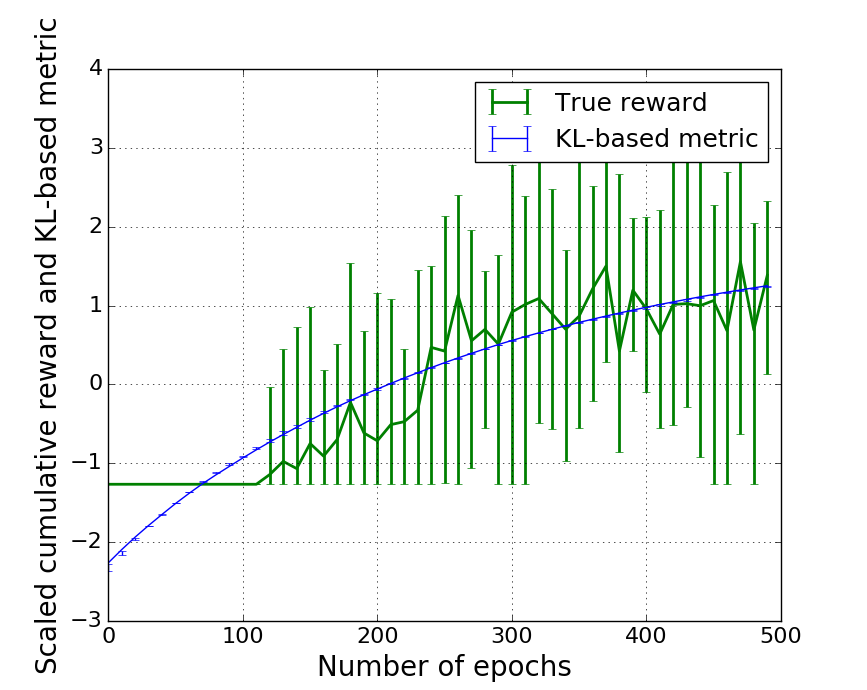
\includegraphics[width=0.15\textwidth]{../misc/mountaincar_correlation.png}
      };
    \end{scope}
    \begin{scope}[xshift=0.13\textwidth]
      \node [mybox] (box){
        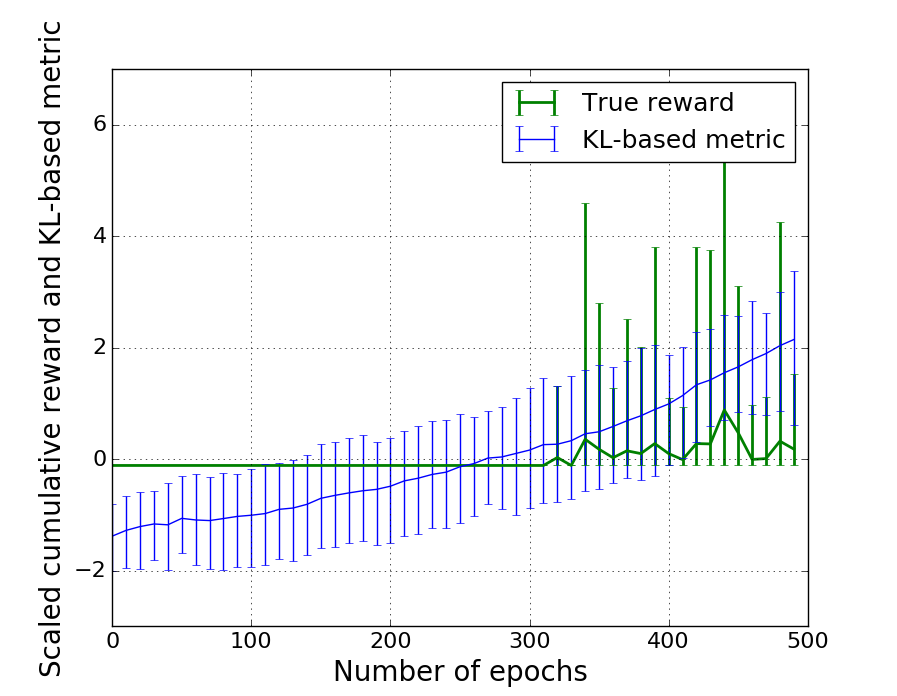
\includegraphics[width=0.15\textwidth]{../misc/mountaincar_correlation_badagent.png}
      };
    \end{scope}
  \end{scope}
  \begin{scope}[yshift=-0.08\textwidth]
    \begin{scope}[xshift=0cm]
        \node[inner sep=0,text width=0.13\textwidth, text centered] (note1) at (0,0) {
         Environment and information gain rewards for a good agent\ldots};
     \end{scope}
    \begin{scope}[xshift=0.14\textwidth]
        \node[inner sep=0,text width=0.13\textwidth, text centered] (note1) at (0,0) {
         Environment and information gain rewards for a bad agent};
     \end{scope}
  \end{scope}
\end{tikzpicture}

\end{center}


\vspace{2\baselineskip}


\mysection{Cumulative surrogate and true environment rewards}

\begin{center}
\input{../misc/cumulative_rewards.tex}
\end{center}


\mysection{What we gain with surrogate rewards}

\vspace{0\baselineskip}

{\Large

\begin{itemize}
\item To alleviate the problem of sparse rewards, the reinforcement learning agents are augmented with surrogate rewards. 
\item This helps the bandit framework to select the best agents early, since these rewards are smoother and less sparse than the environment reward. 
\end{itemize}

}


\newpage

\mysection{Frequency of selections of the different agents}

\vspace{0.5\baselineskip}

\begin{center}
  \input{../misc/freq_selection.tex}
\end{center}

\vspace{\baselineskip}

\vspace{0.5\baselineskip}

\mysection{Score for DQN, Gorila, pro human gamer, and the agent selected from the bandit}

  \centering
  \begin{tabular}{|p{5.5cm}|p{6.5cm}|l|p{4.5cm}|p{7.5cm}|}
  \hline
  Games & DQN Score & Gorila Score & Human Pro Score & Best Agent Score\\
  \hline
    Atlantis            & 85641 $\pm$ 17600 & 100069.16 & 29028 & 217810 $\pm$ 7256.4 \\
    Kung-Fu             & 23270 $\pm$  5955 & 27543.33  & 22736 & 29860  $\pm$  6793.1 \\
    Ms. Pacman          &  2311 $\pm$   525 & 3233.50   & 15693 & 5708.0 $\pm$  860.1 \\
    Seaquest            &  5286 $\pm$  1310 & 13169.06  & 20182 & 17214  $\pm$ 2411.5 \\
    Sp. Invaders        &  1976 $\pm$   893 & 1883.41   &  1652 & 3697.5 $\pm$ 2876.1 \\
    Zaxxon              &  4977 $\pm$  1235 & 7129.33   &  9173 & 30610  $\pm$ 8169.0 \\
  \hline  
  \end{tabular}
  \label{tab:1}



\mysection{Conclusions}

{\Large

\begin{itemize}
\item Introduced a bandit framework that offers a principled way of selecting between different RL agent architectures 
\item Maximizing rewards during the learning process
\item Reliably select the best agent (in future expected rewards) 
\item Composite surrogate reward captures the certainty of the agents regarding the environment dynamics, for a given amount of environment interactions.
\item Experimental results show that the bandit outperforms both a single non-optimal agent and uniform alternation between the agents.
\end{itemize}

}

%\small{
%\bibliographystyle{unsrt}
%\bibliographystyle{../misc/natbib}
%\bibliography{../misc/library,../misc/biblio,../misc/bibdesk-porbanz}
%}

\end{multicols}

\end{poster}

\end{document}
